%================================================================
% SLO
%----------------------------------------------------------------
% datoteka: 	thesis_template.tex
%
% opis: 		predloga za pisanje diplomskega dela v formatu LaTeX na
% 				Univerza v Ljubljani, Fakulteti za računalništvo in informatiko
%
% pripravili: 	Matej Kristan, Zoran Bosnić, Andrej Čopar, 
%			  	po začetni predlogi Gašperja Fijavža
%
% popravil: 	Domen Rački
%
% verzija: 		1. april 2015
%================================================================
% ENG
%----------------------------------------------------------------
% file: 		thesis_template.tex
%
% description:	template file for writing the diploma thesis in LaTeX format at
% 				University of Ljubljana, Faculty of Computer and Information Science
%
% prepared by: 	Matej Kristan, Zoran Bosnić, Andrej Čopar, 
%				after the initial template from Gašper Fijavž
%
% edited by:	Domen Rački
%
% version: 		1. april 2015
%================================================================





%================================================================
% SLO: definiraj strukturo dokumenta
% ENG: define file structure
%================================================================
\documentclass[a4paper, 12pt]{book}

%----------------------------------------------------------------
% |||||||||||||||||||||| USTREZNO POPRAVI |||||||||||||||||||||||
% |||||||||||||||||||||| EDIT ACCORDINGLY |||||||||||||||||||||||
%----------------------------------------------------------------
% SLO: definiraj metapodatke za datoteko thesis_template.tex
% ENG: define metadata for the file thesis_template.tex
%----------------------------------------------------------------
\usepackage{filecontents}
\begin{filecontents*}{\jobname.xmpdata}
	\Author{Gregor Majcen}
	\Title{Interaktivne računalniške umetniške instalacije v času hitrega tehnološkega razvoja} 
	\Keywords{
		računalnik\sep
		umetnost\sep 
		pametni telefon\sep 
		android\sep 
		filter\sep 
		digitalna umetnost\sep 
		ohranjanje\sep 
		vzdrževanje programske opreme\sep 
	} 
	\Org{Univerza v Ljubljani, Fakulteta za računalništvo in informatiko}
\end{filecontents*}
% NOTE: the command \Subject is avoided in the given example since there are persisting problems with it
% NOTE: if you have errors conserning ICC profiles, read the pdfx package description file pdfx.pdf, section 'Color profiles'
%----------------------------------------------------------------
% |||||||||||||||||||||| USTREZNO POPRAVI |||||||||||||||||||||||
% |||||||||||||||||||||| EDIT ACCORDINGLY |||||||||||||||||||||||
%----------------------------------------------------------------

%================================================================
% SLO: vključi oblikovanje in pakete
% ENG: include design and packages
%================================================================
%----------------------------------------------------------------
% SLO: generiranje PDFjev iz pdftex, skladnih s PDF/A
% ENG: generating PDF/A compliant PDFs from pdftex
%----------------------------------------------------------------
\usepackage[a-1b]{pdfx}
%----------------------------------------------------------------
% SLO: LaTeX paketi
% ENG: LateX packages
%----------------------------------------------------------------
% SLO: omogoča uporabo slovenskih (latinskih) črk kodiranih v formatu UTF-8
% ENG: enables the use of slovene (latin) caracters encoded in the UFT-8 format
\usepackage[utf8x]{inputenc}   
% SLO: naloži, med drugim, slovenske delilne vzorce
% ENG: loads, among others, slovene dividing patterns
\usepackage[slovene,english]{babel} 
% SLO: poskrbi za postavitev strani
% ENG: takes care of the page layout
\usepackage{fancyhdr}
% SLO: za vlaganje slik različnih formatov
% ENG: for loading figures of different formats
\usepackage{graphicx}
\usepackage{caption}
\captionsetup[figure]{labelfont=bf} % SLO: napis "Slika #" v krepkem tisku
									% ENG: wirte "Figure #" caption in bold
\captionsetup[table]{labelfont=bf} % SLO: napis "Tabela #" v krepkem tisku
								   % ENG: wirte "Table #" caption in bold
% SLO: za pisanje psevdokode
% ENG: for writing pseudocode
\usepackage{algorithm}
\usepackage{algorithmic}
\floatname{algorithm}{\footnotesize Algorithm} % SLO: napis "Algoritem #" v krepkem tisku
											   % ENG: write "Algorithm #" caption in bold
% SLO: poveže reference slik/tabel in slike/tabele znotraj dokumenta
% ENG: links image/table references with the images/tables within the document
\usepackage{hyperref}
% SLO: pri kliku na referenco slike/tabele se postavi na vrh slike/tabele
% ENG: when clicking the image/table reference, position the focus on top of the image/table
\usepackage[all]{hypcap}
% SLO: omogoča, med drugim, definicjo in uporebo barve
% ENG: enables, among others, the definition and use of colors
\usepackage{xcolor}
%----------------------------------------------------------------
% SLO: dodatni paketi
% ENG: additional packages
%----------------------------------------------------------------
% SLO: omogoča večjo manipulacijo nad tabelami
% ENG: allows for greater manipulation of tables
\usepackage{booktabs}
% SLO: naloži dodatne simbole
% ENG: loads additional symbols
\usepackage{amssymb} 
% SLO: omogoča, med drugim, sklicevanje na formule z eqref
% ENG: enables, among others, equation referencing with eqref
\usepackage{amsmath}
% SLO: omogoča komentiranje večjega dela teksta
% ENG: enables the commenting of larger text parts
\usepackage{verbatim}
% SLO: omogoča rotacijo PDF strani v ležeč položaj
% ENG: enables the rotation of a PDF page to landscape
\usepackage{pdflscape}
% SLO: omogoča barvanje vrstic in stolpcev tabel
% ENG: enables coloring of table rows and columns
\usepackage{colortbl}



%================================================================
% SLO: nastavitve dokumenta
% ENG: document properties
%================================================================
% SLO: prilagoditev robov za tisk
% ENG: margin adjustments for printing
\addtolength{\marginparwidth}{-20pt}
\addtolength{\oddsidemargin}{40pt}
\addtolength{\evensidemargin}{-40pt}
% SLO: razmik med vrsticami
% ENG: line spacing
\renewcommand{\baselinestretch}{1.3} 
% SLO: postavitev strani
% ENG: page layout
\renewcommand{\chaptermark}[1]{\markboth{\MakeUppercase{\thechapter.\ #1}}{}} 
\renewcommand{\sectionmark}[1]{\markright{\MakeUppercase{\thesection.\ #1}}} 
\renewcommand{\headrulewidth}{0.5pt} % Header rule
\renewcommand{\footrulewidth}{0pt} % Footer rule
%
\fancypagestyle{frontmatter}{%
	\fancyhf{} % Clear all headers and footers first
	\fancyhead[LE,RO]{\sl \thepage} 
	%\fancyhead[LO]{\sl \rightmark} 
	%\fancyhead[RE]{\sl \leftmark}
}
\fancypagestyle{mainmatter}{%
  	\fancyhf{} % Clear all headers and footers first
	\fancyhead[LE,RO]{\sl \thepage} 
	\fancyhead[LO]{\sl \rightmark} 
	\fancyhead[RE]{\sl \leftmark}
}
% SLO: font za ime avtorja
% ENG: font for author name
\newcommand{\authorfont}{\Large}
% SLO: font za naslov diplomskega dela
% ENG: font for thesis title
\newcommand{\titlefont}{\LARGE\bf}
% SLO: globina kazala
% ENG: content depth
\setcounter{tocdepth}{1}
% SLO: definiraj ukaz za prazno stran
% ENG: define the command for empty page
\newcommand{\clearemptydoublepage}{\newpage{\pagestyle{empty}\cleardoublepage}}

%================================================================
% SLO: razno
% ENG: other
%================================================================
% SLO: nastavitev sklicevanj
% ENG: hyper referencing setup
\definecolor{black}{rgb}{0,0,0}
\hypersetup{
	colorlinks = true,
	linkcolor = black,
	citecolor = black,
	urlcolor = black
}
%----------------------------------------------------------------
% |||||||||||||||||||||| USTREZNO POPRAVI |||||||||||||||||||||||
% |||||||||||||||||||||| EDIT ACCORDINGLY |||||||||||||||||||||||
%----------------------------------------------------------------
\newcommand{\myname}{Gregor Majcen}
\newcommand{\mytitle}{Interaktivne računalniške umetniške instalacije v času hitrega tehnološkega razvoja}
\newcommand{\myyear}{2015}
\newcommand{\mysupervisor}{prof.~dr.\ Franc Solina}
%----------------------------------------------------------------
% SLO: dodaj poti do datotek s slikami, tabelami, ...
% ENG: add paths to files containing figures, tables, ...
%----------------------------------------------------------------
\graphicspath{
	{./figures/}
	{./tables/}
}
%----------------------------------------------------------------
% SLO: moji paketi
% ENG: my packages
%----------------------------------------------------------------
% ...
%----------------------------------------------------------------
% SLO: moji konstrukti
% ENG: my constructs
%----------------------------------------------------------------
\newtheorem{izrek}{Izrek}[chapter]
\newtheorem{trditev}{Trditev}[izrek]
\newenvironment{dokaz}{\emph{Dokaz.}\ }{\hspace{\fill}{$\Box$}}
\newcommand{\BibTeX}{{\sc Bib}\TeX}
%----------------------------------------------------------------
% |||||||||||||||||||||| USTREZNO POPRAVI |||||||||||||||||||||||
% |||||||||||||||||||||| EDIT ACCORDINGLY |||||||||||||||||||||||
%----------------------------------------------------------------





%================================================================
% SLO: začetne strani diplomskega dela
% ENG: fist pages of the diploma thesis
%================================================================
\begin{document}
% SLO: prepreči težave s številkami strani v kazalu
% ENG: prevents problems with the page numbers in the contents page
\renewcommand{\thepage}{}

%----------------------------------------------------------------
% SLO: naslovnica (vstavi naslovnico (LaTeX kodo) iz datoteke pages/title.tex)
% ENG: title page (insert the title page (LaTeX code) from the file pages/title.tex)
%----------------------------------------------------------------
\thispagestyle{empty}
	\begin{center}
        {\large\sc Univerza v Ljubljani\\Fakulteta za računalništvo in informatiko}
    	\vskip 10em
    	{\authorfont \myname \par}
    	{\titlefont \mytitle \par}
    {\vskip 2em \textsc{MAGISTRSKO DELO\\[2mm]
    ŠTUDIJSKI PROGRAM DRUGE STOPNJE\\RAČUNALNIŠTVO IN INFORMATIKA}\par}
    \vfill\null
    {\large \textsc{Mentor}: \mysupervisor \par}
    {\vskip 2em \large Ljubljana, \myyear \par}
\end{center} \clearemptydoublepage 
%\thispagestyle{empty}
	\begin{center}
        {\large\sc University of Ljubljana\\Faculty of Computer and Information Science}
    	\vskip 10em
    	{\authorfont \myname \par}
    	{\titlefont \mytitle \par}
    {\vskip 2em \textsc{MASTERS THESIS\\[2mm]
    THE 2nd CYCLE MASTERS STUDY PROGRAMME\\COMPUTER AND INFORMATION SCIENCE}\par}
    \vfill\null
    {\large \textsc{Supervisor}: \mysupervisor \par}
   	{\large \textsc{Co-supervisor}:  \mycosupervisor \par}
    {\vskip 2em \large Ljubljana, \myyear \par}
\end{center} \clearemptydoublepage

%----------------------------------------------------------------
% SLO: avtorske pravice
% ENG: copyright
%----------------------------------------------------------------
\thispagestyle{empty}
\vspace*{\fill}
{\noindent\footnotesize
{\sc Avtorske pravice}. Rezultati magistrskega dela so intelektualna lastnina avtorja in Fakultete za ra\-ču\-nal\-niš\-tvo in informatiko Univerze v Ljubljani. Za objavljanje ali izkoriščanje rezultatov ma\-gi\-str\-ske\-ga dela je potrebno pisno soglasje avtorja, Fakultete za ra\-ču\-nal\-niš\-tvo in informatiko ter mentorja.}
\begin{center}
{\footnotesize{\sc \copyright \myyear\ \myname}}
\end{center} \clearemptydoublepage
%\thispagestyle{empty}
\vspace*{\fill}
{\noindent\footnotesize
{\sc Copyright}. The results of this Masters Thesis are the intellectual property of the author and the Faculty of Computer and Information Science, University of Ljubljana. For the publication or exploitation of the Masters Thesis results, a written consent of the author, the Faculty of Computer and Information Science, and the supervisor is necessary.}
\begin{center}
{\footnotesize{\sc \copyright \myyear\ \myname}}
\end{center} \clearemptydoublepage

%----------------------------------------------------------------
% SLO: izjava o avtorstvu
% ENG: declaration of authorship
%----------------------------------------------------------------
\vspace*{1cm}
\begin{center}
{\Large \textbf{\sc Izjava o avtorstvu magistrskega dela}}
\end{center}

\vspace{1cm}
\noindent Spodaj podpisani \myname\ sem avtor magistrskega dela z naslovom:

\vspace{0.5cm}
\begin{center}
\emph{\mytitle}
\end{center}

\vspace{1cm}
\noindent S svojim podpisom zagotavljam, da:
\begin{itemize}
    \item sem magistrsko delo izdelal samostojno pod mentorstvom prof.~dr.\ Franca Soline,

    \item so elektronska oblika magistrskega dela, naslov (slovenski, angleški), povzetek (slovenski, angleški) ter ključne besede (slovenske, angleške) identični s tiskano obliko magistrskega dela,
    \item soglašam z javno objavo elektronske oblike magistrskega dela v zbirki ``Dela FRI''.
\end{itemize}

\vspace{1cm}
\noindent V Ljubljani, 13. avgusta 2015 \hfill Podpis avtorja:
 \clearemptydoublepage
%\vspace*{1cm}
\begin{center}
{\Large \textbf{\sc Declaration of Masters Thesis authorship}}
\end{center}

\vspace{1cm}
\noindent I, the undersigned \myname\ am the author of the Master Thesis entitled:

\vspace{0.5cm}
\begin{center}
\emph{\mytitle}
\end{center}

\vspace{1cm}
\noindent With my signature, I declare that:
\begin{itemize}
	\item the submitted Thesis is my own unaided work under the supervision of \mysupervisor\ and co-supervision of \mycosupervisor,

	\item all electronic forms of the Masters Thesis, title (Slovenian, English), abstract (Slovenian, English) and keywords (Slovenian, English) are identical to the printed form of the Masters Thesis,
	\item I agree with the publication of the electronic form of the Masters Thesis in the collection ''Dela FRI''. 
\end{itemize}

\vspace{1cm}
\noindent In Ljubljana, 3. April 2015 \hfill Author's signature: \clearemptydoublepage

%----------------------------------------------------------------
% SLO: zahvala
% ENG: acknowledgements
%----------------------------------------------------------------
\thispagestyle{empty}

\begin{center}
{\Large \textbf{\sc Zahvala}}
\end{center}
\vspace{0.5cm}

{\it\noindent
Hvala mentorju prof. dr. Francu Solini za vso strokovno pomoč in material za izdelavo magistrskega dela.

Hvala neuradnemu somentorju viš. pred. dr. Borutu Batagelju za pomoč tako pri izdelavi praktičnega dela magistrskega dela kot tudi pri dobavi strojne opreme.

Največja zahvala gre ženi Mateji za spodbudo, podporo in zabavo, ki je nastala med testiranjem praktičnega dela.

Hvala tudi moji in ženini družini za vso spodbudo, da zmorem.

Hvala prijatelju in sodelavcu Maticu Potočniku za komentarje, ideje in debate o tem, kaj vse bi se iz te naloge še dalo narediti.

Hvala tudi Teji, ki je to delo lektorirala, da branje lepše in lažje teče.

\vspace{0.5cm} \hfill \myname, \myyear
}
 \clearemptydoublepage
%\thispagestyle{empty}

\begin{center}
{\Large \textbf{\sc Acknowledgments}}
\end{center}
\vspace{0.5cm}

{\it\noindent
Worth mentioning in the acknowledgment is everyone who contributed to your thesis.

\vspace{0.5cm} \hfill \myname, \myyear
} \clearemptydoublepage

%----------------------------------------------------------------
% SLO: kazalo
% ENG: contents
%----------------------------------------------------------------
\begingroup
	\hypersetup{colorlinks=true,linkcolor=black}
	\def\thepage{}
	\tableofcontents{}
	\clearemptydoublepage
\endgroup



%================================================================
% SLO: glavne strani diplomskega dela
% ENG: main pages of the diploma thesis
%================================================================
% SLO: izklopi številčenje poglavji in uporabi rimskime številkami za številke strani
% ENG: turns off chapter numbering and uses roman numerals for page numbers
\frontmatter 
\pagestyle{frontmatter}


	
%---------------------------------------------------------------
% SLO: slovenski povzetek
% ENG: slovenian abstract
%---------------------------------------------------------------
\selectlanguage{slovene} % Preklopi na slovenski jezik
\chapter{Povzetek}

V vzorcu je predstavljen postopek priprave magistrskega dela z uporabo okolja \LaTeX. Vaš povzetek mora sicer vsebovati približno 100 besed, ta tukaj je odločno prekratek. Dober povzetek vključuje: (1) kratek opis obravnavanega problema, (2) kratek opis vašega pristopa za reševanje tega problema in (3) (najbolj uspešen) rezultat ali prispevek magistrske naloge.

\subsection*{Ključne besede}
\textit{beseda1, beseda2, beseda3}
\clearemptydoublepage



%---------------------------------------------------------------
% SLO: angleški povzetek
% ENG: english abstract
%---------------------------------------------------------------
\selectlanguage{english} % Preklopi na angleški jezik
\chapter{Abstract}

This sample document presents an approach to typesetting your BSc thesis using \LaTeX. A proper abstract should contain around 100 words which makes this one way too short. A good abstract contains: (1) a short description of the tackled problem, (2) a short description of your approach to solving the problem, and (3) (the most successful) result or contribution in your thesis.

\subsection*{Keywords}
\textit{word1, word2, word3}
\clearemptydoublepage



\selectlanguage{slovene} % Preklopi na slovenski jezik
%================================================================
% SLO: osrednji del naloge
% ENG: main part of the paper
%================================================================
% SLO: vklopi številčenje poglavji, ponastavi številčenje strani in uporabi arabske številkami za številčenje strani
% ENG: turns on chapter numbering, resets page numbering and uses arabic numerals for page numbers
\mainmatter 
\pagestyle{mainmatter}



%----------------------------------------------------------------
% Poglavje 1
%----------------------------------------------------------------
\chapter{Uvod}
\label{ch:uvod}

Datoteka {\tt magistrska\_naloga.tex} na kratko opisuje, kako se pisanja magistrskega dela lotimo z uporabo programskega pateka \LaTeX. V tem dokumentu bomo predstavili nekaj njegovih prednosti in hib. Kar se slednjih tiče, mi pride na misel ena sama. Ko se srečamo z njim, nam izgleda kot kislo jabolko, nismo prepričani, da bi želeli vanj ugrizniti. Lahko pa z njim pripravimo odličen zavitek ali pa pridemo na okus.

Česa od tega dokumenta ne pričakujte? Izkušeni uporabniki \LaTeX{}a bi vse skupaj zastavili
drugače. Morda bi napisali posebno razredno datoteko (\emph{class file}) --- v resnici priredili katero od obstoječih ---, v datoteki {\tt magistrska\_naloga.tex} ohranili samo najbolj grobo strukturo in vanjo vključevali  posamezna po\-glav\-ja. Hkrati s pisanjem teksta bi poskrbeli tudi za stvarno kazalo ({\tt makeindex}), literaturo pa bi citirali z uporabo {\BibTeX}{a}. Tega, skratka, v tem dokumentu ne boste našli.

Kaj vseeno najdemo. V Poglavju~\ref{ch:uvod} bomo na hitro spoznali besedilne konstrukte kot so izreki, enačbe in dokazi. Naučili se bomo, kako se na njih sklicujemo. V Poglavju~\ref{ch:sklicevanje} se bomo srečali s sklicevanjem na besedilne konstrukte. Poglavje~\ref{ch:plovke} bo predstavilo vključevanje plovk: slik in tabel.
Razni drugi napotki so dani v Poglavju~\ref{ch:razno}.

\chapter{Sklicevanje na besedilne konstrukte}
\label{ch:sklicevanje}

Matematična ali popolna indukcija je eno prvih orodij, ki jih spoznamo za dokazovanje trditev pri matematičnih predmetih.
\begin{izrek}
\label{iz:1}
Za vsako naravno število $n$ velja
\begin{equation}
n < 2^n.
\label{eq:1}
\end{equation}
\end{izrek}
\begin{dokaz}
Dokazovanje z indukcijo zahteva, da neenakost~\eqref{eq:1} najprej preverimo za najmanjše naravno število --- $0$. Res, ker je $0 < 1 = 2^0$, je neenačba~\eqref{eq:1} za $n=0$ izpolnjena.

Sledi indukcijski korak. S predpostavko, da je neenakost~\eqref{eq:1} veljavna pri nekem naravnem številu $n$, je potrebno pokazati, da je ista neenakost v veljavi tudi pri njegovem nasledniku --- naravnem številu $n+1$. Računajmo.
\begin{align}
n+1 &< 2^n + 1  \label{eq:2}\\
    &\le 2^n + 2^n \label{eq:3}\\
    &= 2^{n+1} \nonumber
\end{align}
Neenakost~\eqref{eq:2} je posledica indukcijske predpostavke, neenakost~\eqref{eq:3} pa enostavno dejstvo, da je za vsako naravno število $n$ izraz $2^n$ vsaj tako velik kot 1. S tem je dokaz Izreka~\ref{iz:1} zaključen.
\end{dokaz}

Opazimo, da je \LaTeX\ številko izreka podredil številki poglavja.



%----------------------------------------------------------------
% Poglavje 2
%----------------------------------------------------------------
\chapter{Plovke: slike in tabele}
\label{ch:plovke}

Slike in daljše tabele praviloma vključujemo v dokument kot plovke. Pozicija plovke v končnem izdelku ni pogojena s tekom besedila, temveč z izgledom strani. \LaTeX\ bo skušal plovko postaviti samostojno, praviloma na vrh strani, na kateri se na takšno plovko prvič sklicujemo. Pri tem pa bo na vsako stran končnega izdelka želel postaviti tudi sorazmerno velik del besedila. V skrajnem primeru, če imamo res preveč plovk, se bo odločil za stran popolnoma zapolnjeno s plovkami.

\section{Formati slik}
Bitne slike, vektorske slike, kakršnekoli slike, z \LaTeX{}om lahko vključimo vse.
Slika~\ref{pic1} je v {\tt .pdf} formatu.
\begin{figure}
    \begin{center}
        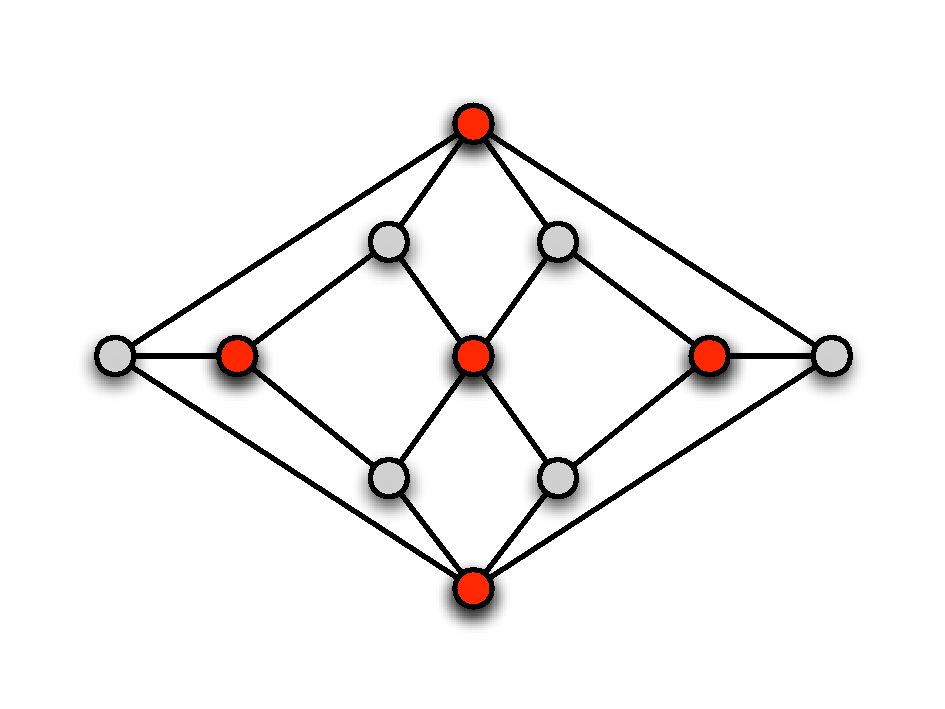
\includegraphics[width=10cm]{pic1.pdf}
    \end{center}
\caption{Herschelov graf, vektorska grafika.}
\label{pic1}
\end{figure}
Pa res lahko vključimo slike katerihkoli formatov? Žal ne. Programski paket \LaTeX\ lahko uporabljamo v več dialektih. Ukaz {\tt latex} ne mara vključenih slik v formatu Portable Document Format {\tt .pdf}, ukaz {\tt pdflatex} pa ne prebavi slik v Encapsulated Postscript Formatu {\tt .eps}.
Strnjeno v Tabeli~\ref{tbl:1}.

\begin{table}
\caption{}
    \begin{center}
        \begin{tabular}{l|ccc}
            ukaz/format & {\tt .pdf} & {\tt .eps} & ostali formati \\ \hline
                        {\tt pdflatex} & da & ne & da \\
                        {\tt latex}   & ne & da  & da
        \end{tabular}
    \end{center}
\label{tbl:1}
\end{table}

Nasvet? Odločite se za uporabo ukaza {\tt pdflatex}. Vaš izdelek bo brez vmesnih stopenj na voljo v {.pdf} formatu in ga lahko odnesete v vsako tiskarno. Če morate na vsak način vključiti sliko, ki jo imate v {\tt .eps} formatu, jo vnaprej pretvorite v alternativni format, denimo {\tt .pdf}.

Včasih se da v okolju za uporabo programskega paketa \LaTeX\ nastaviti na kakšen način bomo prebavljali vhodne dokumente. Spustni meni na Sliki~\ref{pic2} odkriva uporabo \LaTeX{}a v njegovi pdf inkarnaciji --- {\tt pdflatex}.
\begin{figure}
\begin{center}
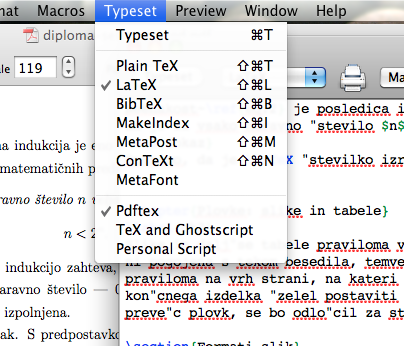
\includegraphics[width=10cm]{pic2.png}
\end{center}
\caption{Kateri dialekt uporabljati?}
\label{pic2}
\end{figure}
Vključena Slika~\ref{pic2} je seveda bitna.



%----------------------------------------------------------------
% Poglavje 3
%----------------------------------------------------------------
\chapter{Razno}
\label{ch:razno}

Primer sklicevanja na literaturo v datoteki {\tt bibliography.bib}. Scale-Invariant Feature Transform (SIFT)~\cite{Lowe}. In kako se sklicujem na več referenc hkrati? Takole:~\cite{Fortnow,Knuth,Lamport,licence}. V~\cite{ubi} pa najdemo podrobnejši opis ter primere uporabe \BibTeX{}a.

\section{Notacije}
\label{sec:notacije}

Za notacijo spremenljivk ter skalarjev uporabimo običajno notacijo, t.j., spremenljivka $x$ in skalar $a$. Pri notaciji matrik ter vektorjev pa se poslužujemo krepega fonta. Torej, matrika $\boldsymbol{A}$ ter vektor $\boldsymbol{v}$,
\begin{equation}
\boldsymbol{A} = \begin{bmatrix}
       a_{11} & a_{12} & \dots & a_{1q}  \\
       a_{21} & a_{22} & \dots & a_{2q}  \\
       \vdots  \\
       a_{p1} & a_{p2} & \dots & a_{pq}  \\
     \end{bmatrix}, \quad
     \boldsymbol{v} = \begin{bmatrix}
       x_1  \\
       x_2  \\
       \vdots  \\
       x_q  \\
     \end{bmatrix}. \nonumber
\end{equation}

%----------------------------------------------------------------
\section{Lepe tabele in psevdokoda}
\label{sec:psevdokoda}

Psevdokoda~\ref{alg:primer} prikazuje primer delovanja genetskega algoritma, medtem ko Tabela~\ref{tab:params} prikazuje primer lepe tabele brez vertikalnih črt. V Dodatku~\ref{ch:dodatek} lahko najdemo primer vstavljanja velike tabele ter primer rotacije lista.

\begin{algorithm}
\caption{Psevdokoda genetskega algoritma}
\label{alg:primer}
\begin{algorithmic}[1]
\footnotesize
\STATE $t \gets 0$
\STATE $InitPopulation[P(t)] \gets$ inicializiraj populacijo
\STATE $EvalPopulation[P(t)] \gets$ evaluiraj populacijo
\REPEAT
\STATE $P'(t) \gets Variation[P(t)] \gets $ generiraj novo populacijo
\STATE $EvalPopulation[P'(t)] \gets$ evaluiraj novo populacijo
\STATE $P(t+1) \gets ApplyGeneticOperators[P'(t) \in Q]$
\STATE $t \gets t+1$
\UNTIL{prekinitev}
\IF{rezultat dovolj dober} 
\STATE shrani rezultat
\ENDIF
\end{algorithmic}
\end{algorithm}

%---------------------------------------------------------------
\begin{table}
\caption{Primer enostavne tabele.}
\centering
\scalebox{0.82}{
\begin{tabular}{c c c}
 \toprule
 Ime & Vrednost & Opis \\
 \midrule
 \textit{ $a$ } & 0.03 &  skalar \\
 \textit{ $x$ } & -1 & spremenljivka \\
 \bottomrule
\end{tabular}
}
\label{tab:params}
\end{table}





%----------------------------------------------------------------
% SLO: bibliografija
% ENG: bibliography
%----------------------------------------------------------------
\bibliographystyle{elsarticle-num}
\bibliography{bibliography}

\begin{comment}
\begin{thebibliography}{99}
\bibitem{lf} L.\ Fortnow, ``Viewpoint: Time for computer science to grow up'',
{\it Communications of the ACM}, št.\ 52, zv.\ 8, str.\ 33--35, 2009.
\bibitem{dk1} D.\ E.\ Knuth, P. Bendix. ``Simple word problems in universal algebras'', v zborniku: Computational Problems in Abstract Algebra (ur. J. Leech), 1970, str. 263--297.
\bibitem{lat} L.\ Lamport. {\it LaTEX: A Document Preparation System}. Addison-Wesley, 1986.
\bibitem{bib} O.\ Patashnik (1998) \BibTeX{}ing.
Dostopno na: \url{http://ftp.univie.ac.at/packages/tex/biblio/bibtex/contrib/doc/btxdoc.pdf}
\bibitem{licence} licence-cc.pdf. Dostopno na: \url{https://ucilnica.fri.uni-lj.si/course/view.php?id=274}
\end{thebibliography}
\end{comment}



%----------------------------------------------------------------
% SLO: priloge
% ENG: appendix
%----------------------------------------------------------------
\appendix
\chapter{Primer vstavljanja velike tabele}
\label{ch:dodatek}

\begin{landscape}
\definecolor{LightGray}{rgb}{0.9412,0.9412,0.9412}
\newcolumntype{a}{>{\columncolor{LightGray}}c}

\begin{table}[ht]
\caption{Primer vključevanja večje tabele v \LaTeX{}.}
\centering
\scalebox{0.48}{
\begin{tabular}{l@{\hspace{4em}}  a c a c a c@{\hspace{4em}}    a c a c a c}
\toprule
 & \multicolumn{6}{c}{$H_{total}$}{\hspace{4em}} & \multicolumn{6}{c}{$H_{\tau_{GHT}}$}\\
 & $\mathcal{B}$ & $\mathcal{B}_\tau$ & $\mathcal{C}^{E}$ & $\mathcal{C}_\tau^{E}$ & $\mathcal{C}^{N}$ & $\mathcal{C}_\tau^{N}$ & $\mathcal{B}$ & $\mathcal{B}_\tau$ & $\mathcal{C}^{E}$ & $\mathcal{C}_\tau^{E}$ & $\mathcal{C}^{N}$ & $\mathcal{C}_\tau^{N}$ \\
\midrule
\input{tables/table_1.txt}
\bottomrule
\end{tabular}
}
\label{tab:tab1}
\end{table}
\end{landscape}


\backmatter
\end{document}
